\documentclass[tikz,border=2mm]{standalone}
\usepackage{tikz}
\usetikzlibrary{arrows.meta, positioning}
\usetikzlibrary{shapes.geometric}
\usetikzlibrary{shapes,arrows.meta,positioning}

\begin{document}

% \hspace{-0.5cm}
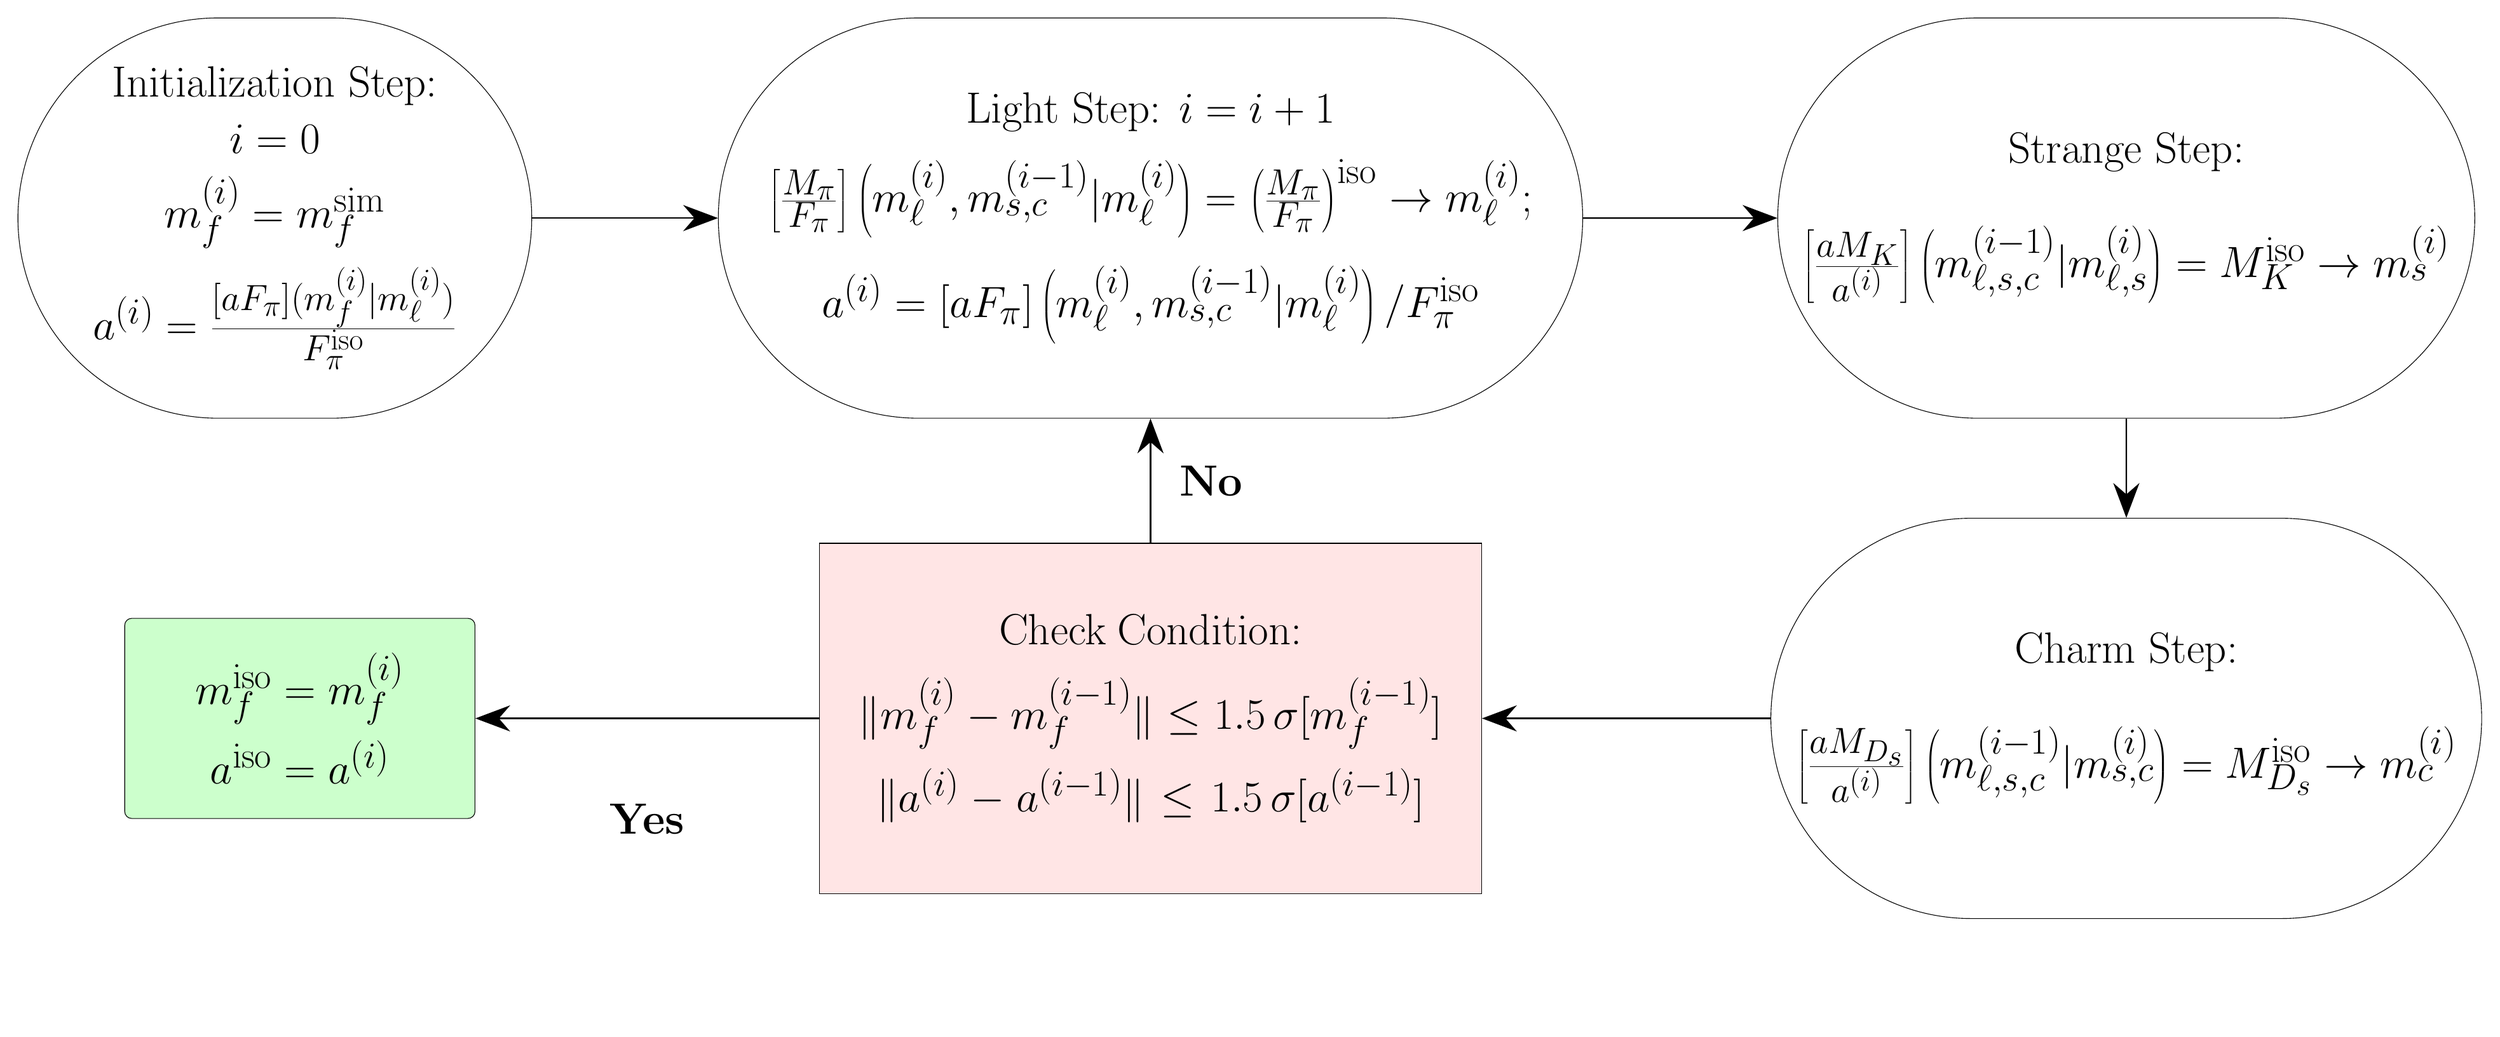
\begin{tikzpicture}[
    node distance=20cm and 12cm, % Further increased horizontal distance between nodes
    every node/.style={draw, minimum height=8.0cm , minimum width=2cm, align=center, font=\large}, % Increased height and width with larger text
    process/.style={rounded rectangle, fill=white},
    lightstep/.style={rounded rectangle, fill=white, draw, minimum height=8.0cm , minimum width=2cm, align=center, font=\Huge}, % Increased height and width with larger text
    decision/.style={rectangle, aspect=2, fill=red!10, text width=13cm, minimum height=7cm, align=center, font=\huge},
    line/.style={draw, -{Stealth[scale=3]}, thick}, % Thicker arrows for better visibility
    iso/.style={draw, rectangle, rounded corners, minimum height=4cm, minimum width=7cm, fill=green!20, font=\large} % Increased height and width of iso result node
]

% Initialization step
\node[process] (init) {\Huge Initialization Step: \\[10pt] \Huge $i = 0$ \\ [12pt]  \Huge $m_f^{(i)} = m^{\rm sim}_{f}$ \\[10pt] \Huge $a^{(i)} = \frac{ [a {F_\pi}](m_f^{(i)}|m_\ell^{(i)})}{F_{\pi}^{\rm iso}}$};

% Light step
\node[lightstep, right of=init, node distance=17.5cm] (light) { \Huge Light Step: $i = i + 1$ \\[15pt]  \Huge $\left[\frac{{M_\pi}}{F_{\pi}}\right]\left(m_{\ell}^{(i)}, m_{s,c}^{(i-1)} \bigg| m_{\ell}^{(i)} \right) = \left(\frac{M_\pi}{F_{\pi}}\right)^{\rm iso} \rightarrow m_\ell^{(i)}$; \\[15pt]
\Huge $a^{(i)} =  [a {F_\pi}]\left(m_{\ell}^{(i)}, m_{s,c}^{(i-1)}\bigg|m_\ell^{(i)}\right)/F_{\pi}^{\rm iso}$};


% Strange step
\node[process, right of=light, node distance=19.5cm] (strange) {\Huge Strange Step: \\[30pt] \Huge $\left[\frac{a{M_K}}{a^{(i)}}\right]\left( m_{\ell,s,c}^{(i-1)} \bigg| m_{\ell,s}^{(i)}  \right) = M_K^{\rm iso} \rightarrow m_s^{(i)}$};

% Charm step
\node[process, below of=strange, node distance=10cm] (charm) { \Huge Charm Step: \\[30pt] \Huge $\left[ \frac{a{M_{D_s}}}{a^{(i)}}\right]\left( m_{\ell,s,c}^{(i-1)} \bigg| m_{s,c}^{(i)} \right) = M_{D_s}^{\rm iso} \rightarrow m_c^{(i)}$};

% Decision: Check condition
\node[decision, left of=charm, node distance=19.5cm] (check) {\Huge Check Condition: \\[18pt] \Huge $\,\,\,\, \|m_f^{(i)} - m_f^{(i-1)}\| \leq 1.5  \, \sigma[ m_f^{(i-1)}]\,\,\,\,$ \\[10pt] \Huge $\,\,\,\, \|a^{(i)} - a^{(i-1)}\| \leq 1.5 \,\sigma[a^{(i-1)}]\,\,\,\,$};

% Iso result (placed below "Check Condition" node)
\node[iso, left of=check, node distance = 17.0cm] (yes) {\Huge $m_f^{\rm iso} = m_f^{(i)}$ \\[8pt] \Huge $a^{\rm iso} = a^{(i)}$};

% Arrows
\path[line] (init) -- (light);
\path[line] (light) -- (strange);
\path[line] (strange) -- (charm);
\path[line] (charm) -- (check);
\path[line] (check) -- node[midway, left=0.1cm, below=-2cm,  font=\bfseries\Huge, draw=none, fill=none] {Yes} (yes); % Place "Yes" label closer to arrow
\path[line] (check.north) to[out=90, in=90, looseness=0] node[midway, above right=-5.5cm, right=0.2cm, font=\bfseries\Huge, draw=none, fill=none] {No} (light.south); % Less bendy arrow connecting "Check Condition" to "Light Step"

\end{tikzpicture}


\end{document}